%%%%%%%%%%%%%%%%%%%%%%%%%%%%%%%%%%%%%%%%%%%%%%%%%%%%%%%%%%%%%%%%%%%%%%%%%%%%%%%
% bt_balazond_slides.tex - Bachelor thesis                                    %
% Subject: bc_emu - portable video game emulator                              %
% Author: Ondrej Balaz <ondra@blami.net>                                      %
%%%%%%%%%%%%%%%%%%%%%%%%%%%%%%%%%%%%%%%%%%%%%%%%%%%%%%%%%%%%%%%%%%%%%%%%%%%%%%%

\documentclass[10pt]{beamer}

% LaTeX packages
\usepackage[czech, english]{babel}
\usepackage[T1]{fontenc}
\usepackage[utf8]{inputenc}
\usepackage{ae,aecompl}
\usepackage{graphicx}
\usepackage{url}
\usepackage{verbatim}
\usepackage{listings}

% CTU Styling
% themes
\useinnertheme{circles}
\usecolortheme{whale}
\usecolortheme{orchid}
\useinnertheme[shadow]{rounded}
\useoutertheme{default}
% beamer colors
\definecolor{beamer@ctufee1}{RGB}{41,111,165}   % light FEE blue
\definecolor{beamer@ctufee2}{RGB}{17,60,94}     % dark FEE blue
% color settings
\setbeamercolor{structure}{fg=beamer@ctufee1}
%\setbeamercolor{titlelike}{parent=structure}
\setbeamercolor{frametitle}{fg=white}
\setbeamercolor{title}{fg=white}
\setbeamercolor{item}{fg=beamer@ctufee1}
\setbeamercolor{footline}{bg=black,fg=white}
% templates
% footer template
\defbeamertemplate*{footline}{fel}
{
	\leavevmode
	\begin{beamercolorbox}[wd=1\paperwidth,ht=3.5ex]{footline}
		\vbox to 3.5ex{
			\vfil
			\hskip 2.5ex
			Snímek: \insertframenumber\,/\,\inserttotalframenumber
			\hfill
			\insertsectionnavigationhorizontal{.5\paperwidth}{\hskip0pt plus1filll}{}
			\vfil}
	\end{beamercolorbox}
}

% -----------------------------------------------------------------------------
% Settings
% -----------------------------------------------------------------------------
\title{Emulátor systému NEC PCEngine}
\subtitle{Baklářská práce}
\author{Ondřej Baláž}
\institute{
	{\em Softwarové technologie a management \\
		obor: softwarové inženýrství \\
	}
	\vglue 5mm
	\includegraphics[width=2cm]{fig/cvut.eps} \\
	Katedra počítačů \\
	Fakulta elektrotechnická \\
	České vysoké učení technické v Praze
}
\date{3. února 2010}

\begin{document}

% -----------------------------------------------------------------------------
% Introduction
% -----------------------------------------------------------------------------
\section{Úvod}

\begin{frame}
\titlepage
\end{frame}

% Implementace
\subsection{Motivace a cíle}
\begin{frame}
\frametitle{Motivace a cíle}
%\begin{block}{Vytyčené cíle}
\begin{itemize}
	\item prostudování architektury systému NEC PCEngine
	\item emulace videoherního systému NEC PCEngine
	\begin{itemize}
		\item emulace procesoru
		\item emulace grafického subsystému
		\item případně emulace zvukového generátoru
	\end{itemize}
	\item přenositelnost kódu
	\begin{itemize}
		\item zatím GNU/Linux a Microsoft Windows
		\item ohled na mobilní zařízení \footnotesize{(Android, Symbian, Nintedo DS,
		...)}
	\end{itemize}
	\item modularita výsledného programu
\end{itemize}
%\end{block}
\end{frame}

\subsection{Emulátor}
\begin{frame}
\frametitle{Emulátor}
\begin{alertblock}{Emulátor}
Nástroj napodobující nejen vnější, ale také vnitřní chování emulovaného
systému. Zpravidla jde o software umožňující spouštění nemodifikovaných
programů pro hardwarově neslučitelný systém.
\end{alertblock}
\vglue 5mm
{\bf Využití emulátorů v praxi:}
\begin{itemize}
	\item vývoj software i hardware {\footnotesize (vestavěné systémy,
	jednočipy)}
	\item zpětná kompatibilita {\footnotesize (Apple, Sony, Nintendo)}
	\item komerční využití {\footnotesize (např. účetnictví Účto, MRP)}
	\item analogie s virtuálními stroji a interpretry
\end{itemize}
\end{frame}

% -----------------------------------------------------------------------------
% NEC PCEngine
% -----------------------------------------------------------------------------
\section{NEC PCEngine}

% Specifikace
\subsection{Specifikace}
\begin{frame}
\frametitle{Systém NEC PCEngine}
NEC PCEngine je videoherní systém 3. generace kompletně vyvinutý firmou NEC v
roce 1987.
\begin{columns}
\column{.60\textwidth}
	\begin{block}{Specifikace}
	\begin{itemize}
		\item hybridní architektura 8/16bit
		\item 8KB RAM a 64KB VRAM
		\item programy uloženy v ROM osazené na výměnných modulech
		\item zvukový a obrazový výstup na televizor
		\begin{itemize}
			\item rozlišení obrazu až 512x240x9 bit
			\item FM syntéza zvuku
		\end{itemize}
		\item 8-mi tlačítkový ovladač
	\end{itemize}
	\end{block}
\column{.40\textwidth}
	\begin{center}
		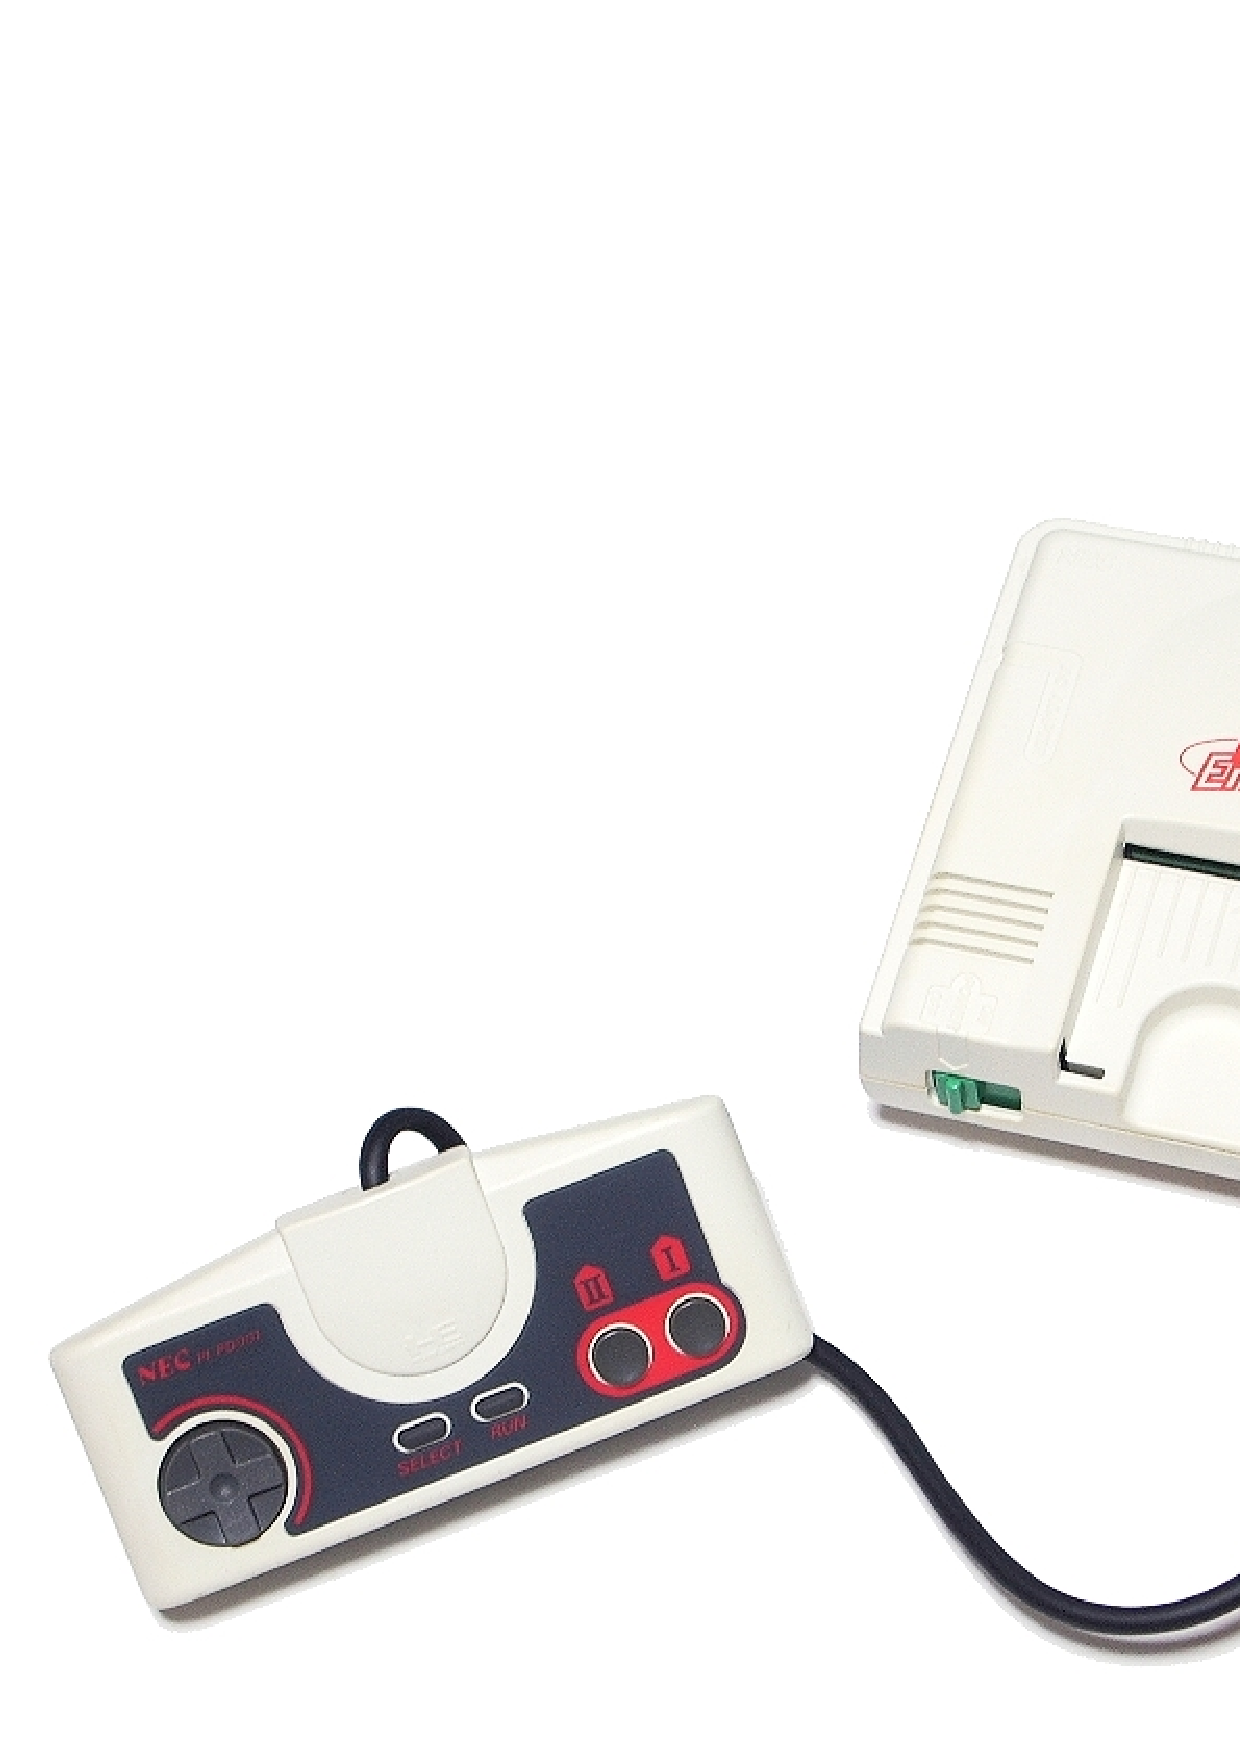
\includegraphics[width=4cm]{fig/pce_photo}
	\end{center}
\end{columns}
\end{frame}

% Architektura
\subsection{Architektura}
\begin{frame}
\frametitle{Architektura systému NEC PCEngine}
Základ systému je tvořen trojicí procesorů propojených řídící sběrnicí.
\vglue 0.15cm
\begin{columns}
\column{.50\textwidth}
	% CPU
	\begin{block}{CPU HuC6280 (8 bit)}
	\begin{itemize}
		\item hlavní procesor
		\item klon WDC 65c02
		\item periferie \\
			PSG, MMU, časovač, ...
	\end{itemize}
	\end{block}
	% VDC
	\begin{block}{VDC HuC6270 (16 bit)}
	\begin{itemize}
		\item grafický koprocesor
	\end{itemize}
	\end{block}
	% VCE
	\begin{block}{VCE HuC6260 (16 bit)}
	\begin{itemize}
		\item enkodér barev
	\end{itemize}
	\end{block}
\column{.50\textwidth}
	\begin{center}
		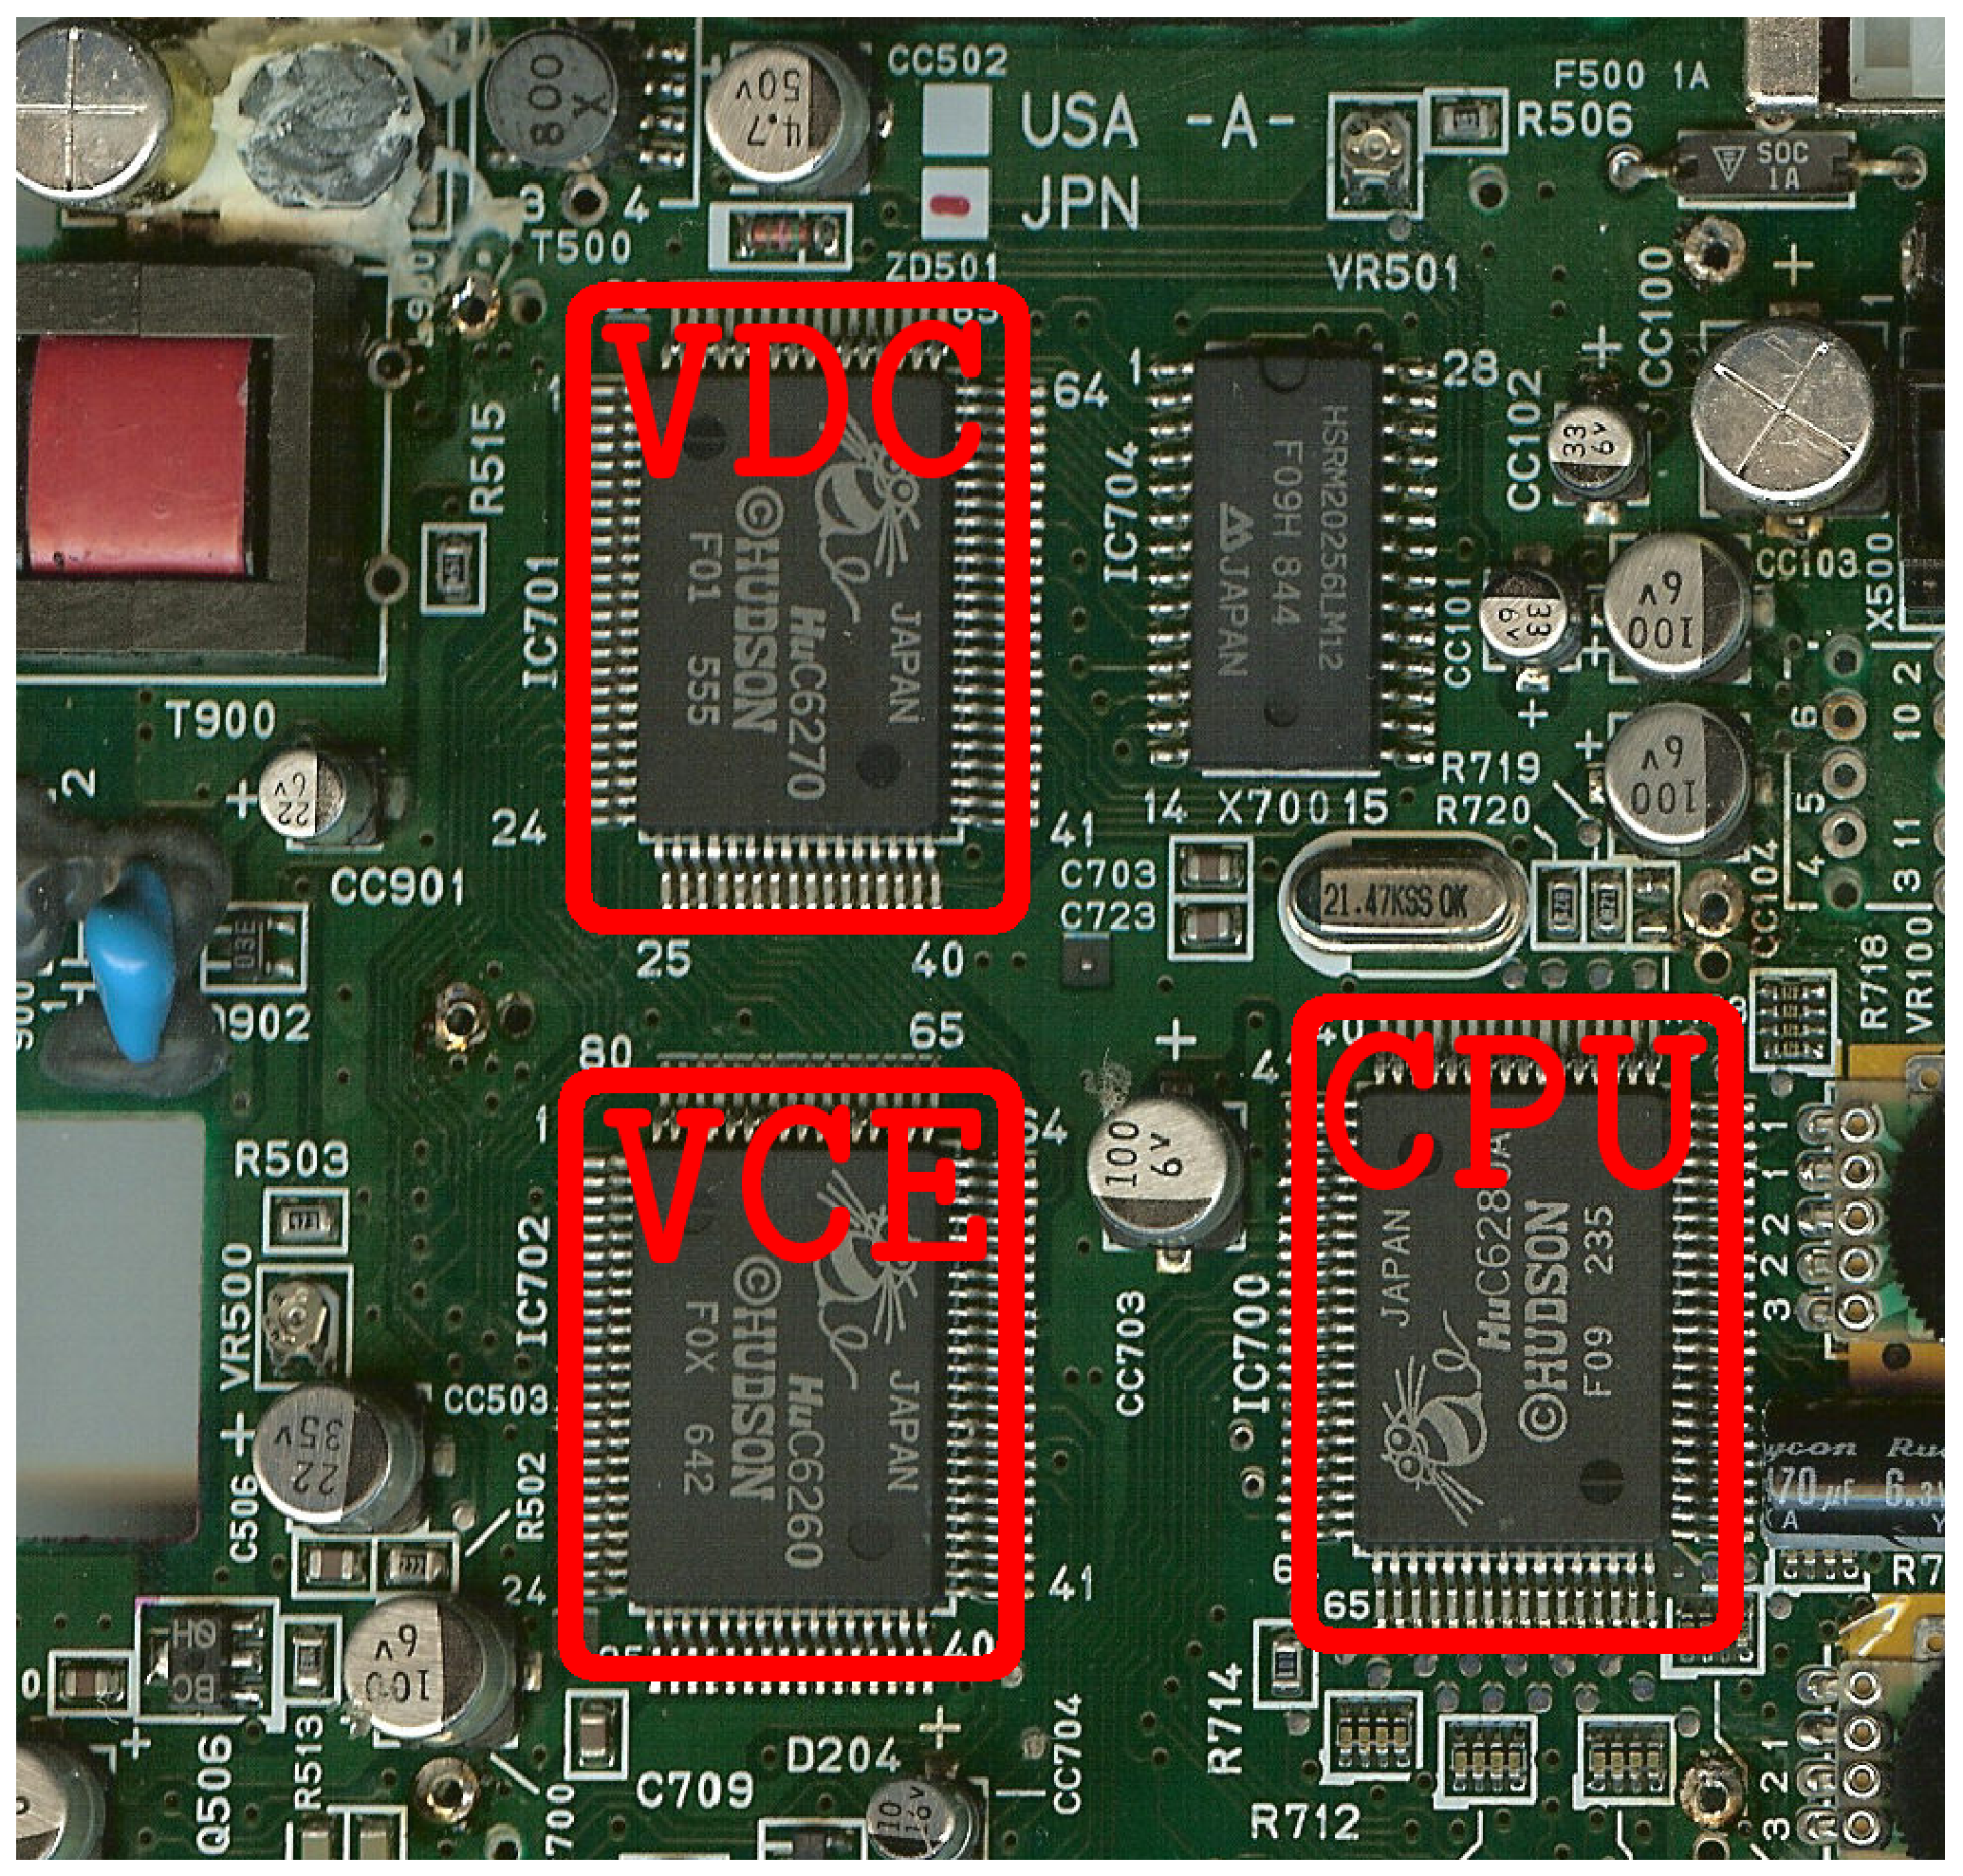
\includegraphics[width=5cm]{fig/pce_board}
	\end{center}
\end{columns}
\end{frame}

\subsection{Speciální vlastnosti systému NEC PCEngine}
\begin{frame}
\frametitle{Speciální vlastnosti systému NEC PCEngine}

\only<1>{
\begin{block}{CPU HuC6280}
\begin{itemize}
	\item veškerá pamět přístupná pouze pomocí 8-mi mapovacích registrů
	\begin{itemize}
		\item lze adresovat až 2 MB fyzické paměti (256 8 KB velkých bank)
		\item fyzická adresa 21 bitů
		\item logická adresa 16 bitů
	\end{itemize}
	\item možnost změny taktovací frekvence za běhu (7.16MHz/3.58MHz)
	\item řada nových instrukcí a adresních módů oproti WDC 65c02
\end{itemize}
\end{block}
\vglue 0.15cm
\begin{center}
	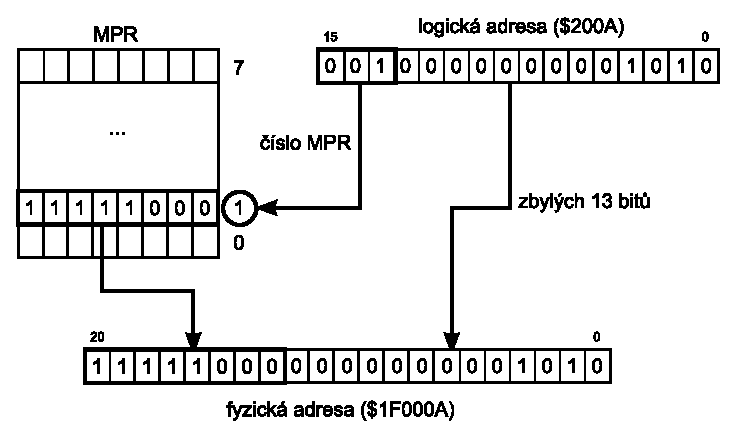
\includegraphics[width=6cm]{fig/pce_banks}
\end{center}
}
\only<2>{
\begin{block}{Grafický systém VDC HuC6270 a VCE HuC6260}
\begin{itemize}
	\item navrženo pro výstup na televizor
	\begin{itemize}
		\item vykreslování po řádcích (tzv. \uv{scanlines})
		\item synchronizace logiky programu pomocí \uv{vertikální synchronizace}
		\item standard NTSC
	\end{itemize}
	\item vzhledem k velikosti VRAM nemá systém {\em framebuffer}
	\item odkazové tabulky deskriptorů {\em BAT} a {\em SAT}
	\item rozdělení obrazu na 2 roviny 
	\begin{itemize}
		\item dlaždice pozadí
		\item sprajty
	\end{itemize}
	\item planární mód uložení obrazových dat
\end{itemize}
\end{block}
}
\end{frame}

% -----------------------------------------------------------------------------
% Implementation
% -----------------------------------------------------------------------------
\section{Implementace}

% Techniky emulace
\subsection{Použité techniky emulace}
\begin{frame}
\frametitle{Použité techniky emulace}
\begin{alertblock}{Interpretační emulace}
Interpretace načtených instrukcí emulovaného programu na datové struktuře
představující procesor.
\end{alertblock}
\vglue 2mm
\begin{columns}
\column{.50\textwidth}
	% Soucasti systemu
	\begin{block}{Paměť}
	\begin{itemize}
		\item prealokované bloky paměti
		\item problém s endianitou $\rightarrow$ {\em union}
	\end{itemize}
	\end{block}
	% Casovani
	\begin{block}{Časování}
	\begin{itemize}
		\item přesnost CPU na cykly
		\item synchronizace CPU cykly/snímek
	\end{itemize}
	\end{block}
\column{.40\textwidth}
	% fig interpretace
	\begin{center}
		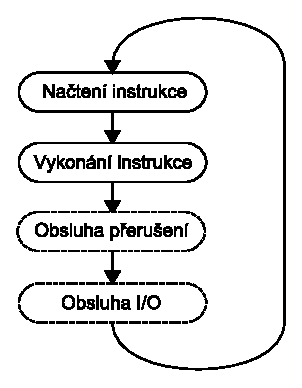
\includegraphics[height=4cm]{fig/anal_interpret}
	\end{center}
\end{columns}
\end{frame}

% Architektura programu
\subsection{Architektura programu}
\begin{frame}
\frametitle{Architektura programu}
\begin{columns}
\column{.50\textwidth}
	\begin{block}{Hlavní myšlenky}
	\begin{itemize}
		\item oddělení logických celků
		\begin{itemize}
			\item uživatelské rozhraní
			\item emulátor
			\item jádro
		\end{itemize}
		\item modularita
		\begin{itemize}
			\item společné rozhraní modulů
			\item přenositelnost
		\end{itemize}
		\item objektový přístup
	\end{itemize}
	\end{block}
\column{.50\textwidth}
	\begin{center}
		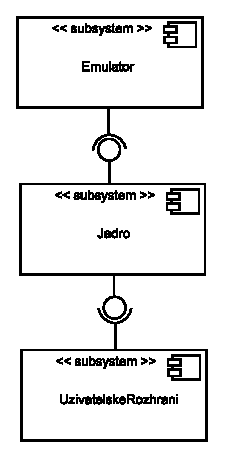
\includegraphics[height=6cm]{fig/anal_kompo}
	\end{center}
\end{columns}
\end{frame}

% -----------------------------------------------------------------------------
% Testing
% -----------------------------------------------------------------------------
\section{Testování}

% 
\subsection{Testování}
\begin{frame}
\frametitle{Lazení a testování}
\begin{block}{Chyby a důležitost lazení a testování}
\begin{itemize}
	\item oficiální dokumentace není dostupná, neoficiální je neúplná s řadou
		nepřesností či chyb
	\item programy využívají chybného chování původního hardware
	\begin{itemize}
		\item je nutné emulovat i chyby původního hardware
	\end{itemize}
	\item interpretační emulátory se ladí \uv{snadno} (datové struktury)
\end{itemize}
\end{block}
\vglue 2.5mm
{\bf Způsob testování naimplementovaného emulátoru:} \\
\begin{itemize}
	\item krátké assemblerové programy pro ověření funkčnosti CPU
	\item obrazy původních programů pořízené pomocí zařízení PCEPro32
	\item volně dostupné \uv{homebrew} programy
\end{itemize}
\end{frame}

% Snimky
\subsection{Snímky obrazovky}
\begin{frame}
\frametitle{Snímky obrazovky}
Fotografie televizoru s výstupem skutečného systému: \\
\vglue 0.1cm
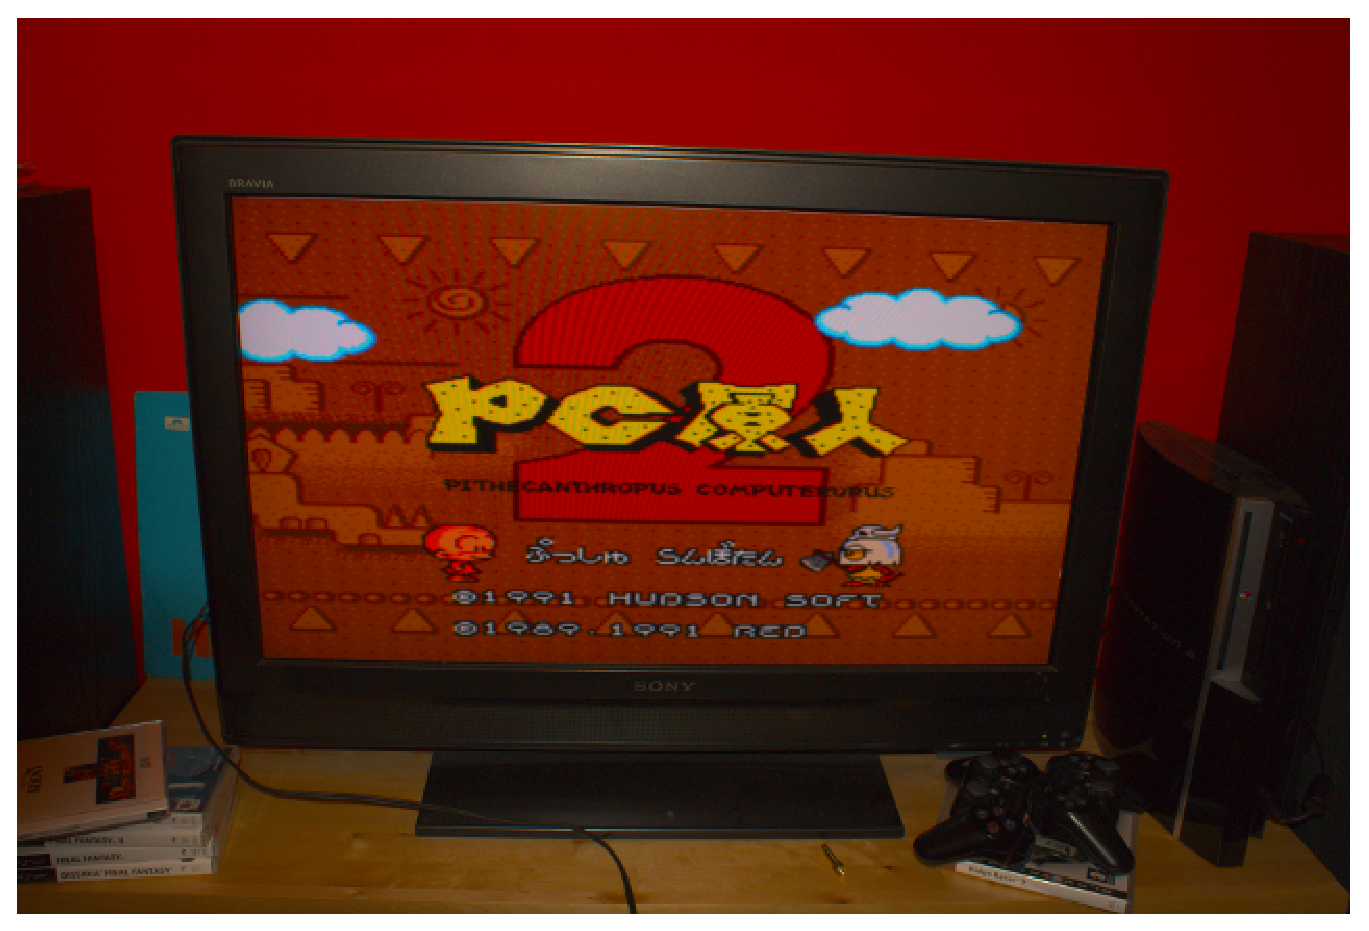
\includegraphics[width=3.6cm]{fig/pce_ss1}
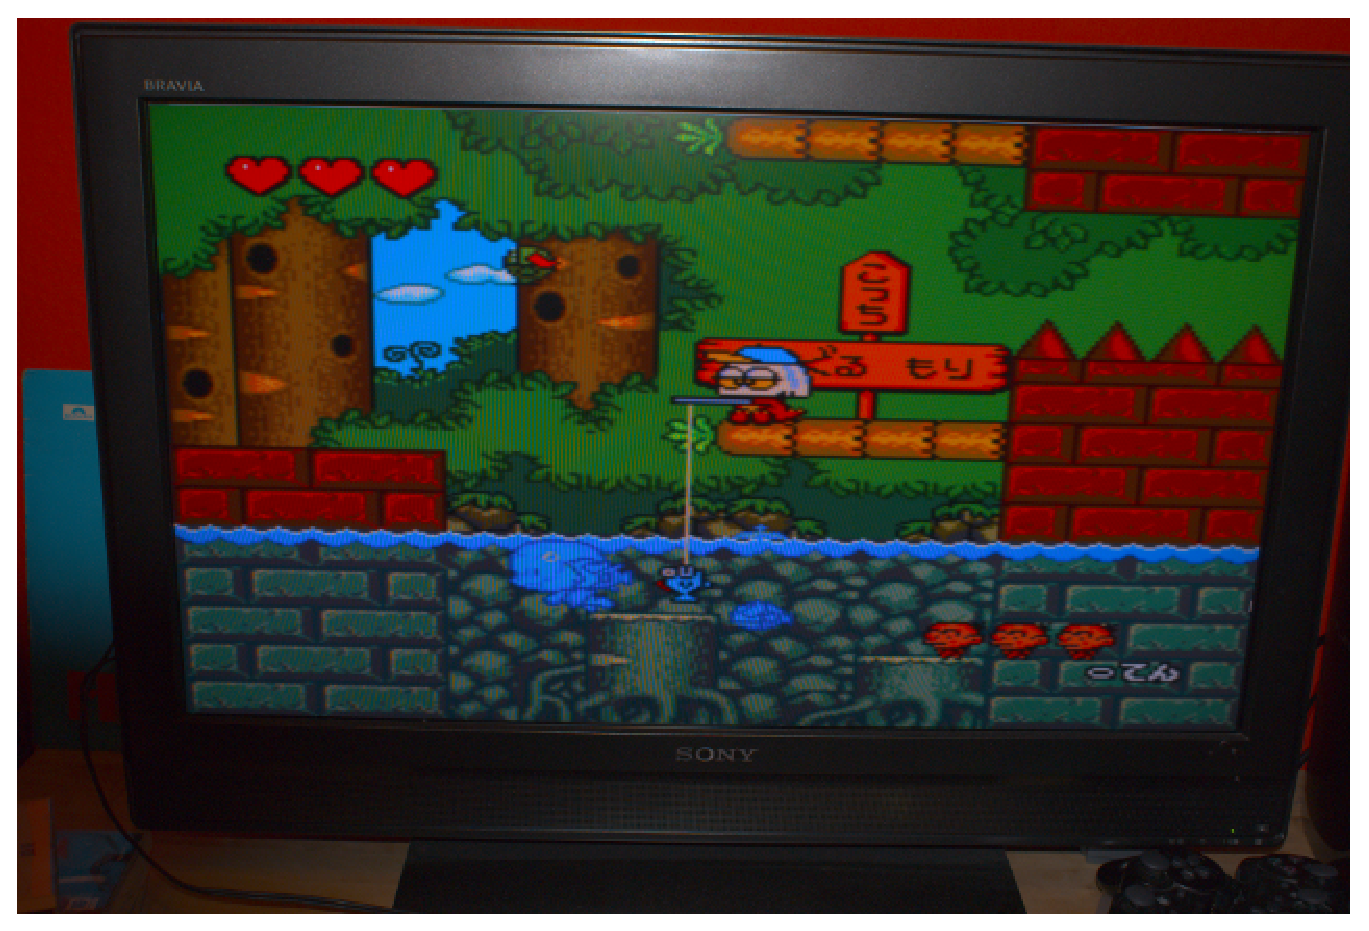
\includegraphics[width=3.6cm]{fig/pce_ss2}
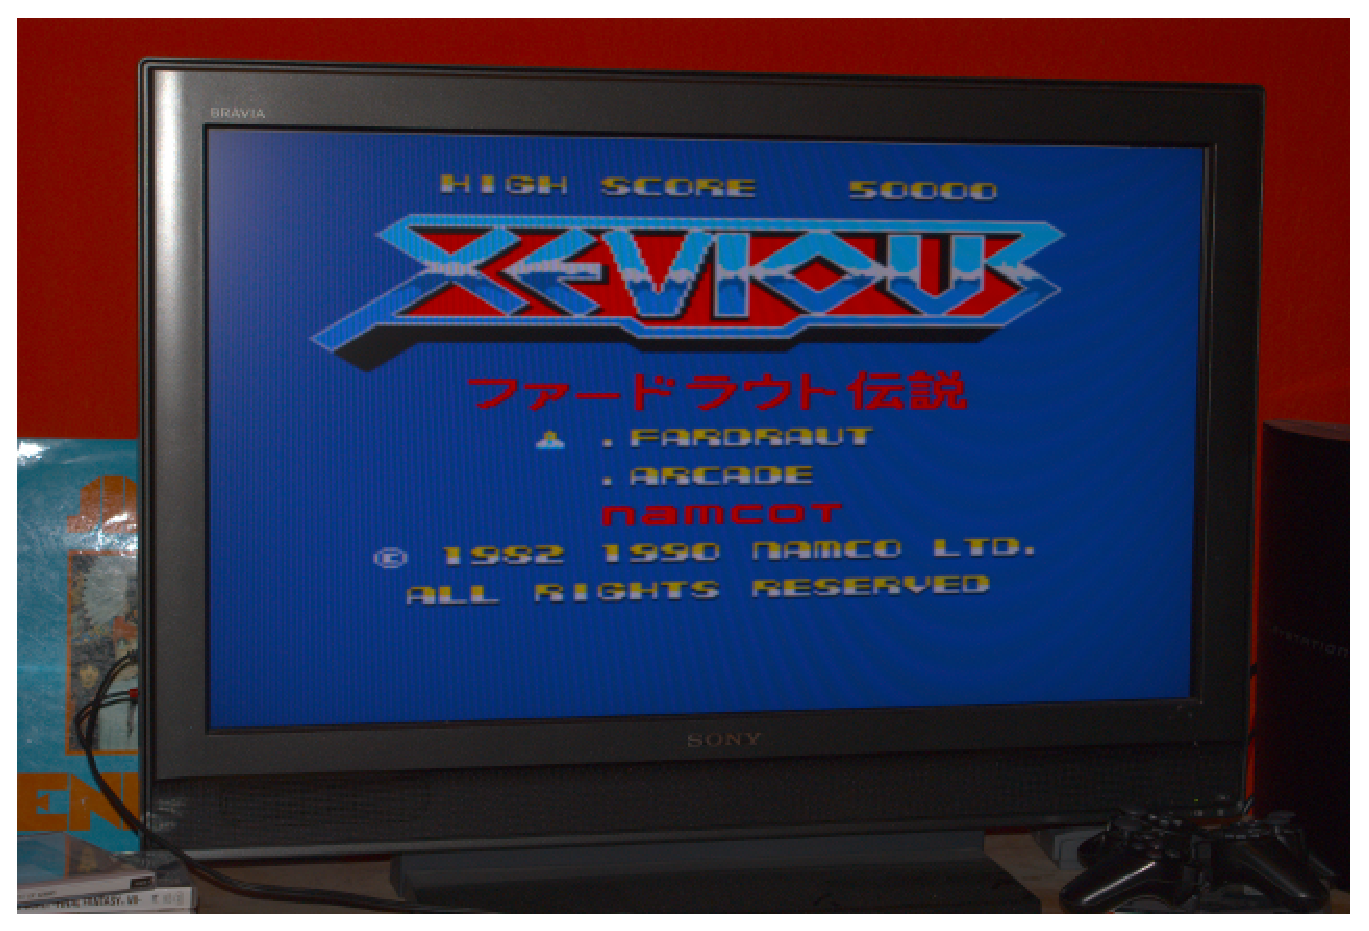
\includegraphics[width=3.6cm]{fig/pce_ss3}
\vglue 0.2cm
Snímky obrazovek stejných programů v emulátoru: \\
\vglue 0.1cm
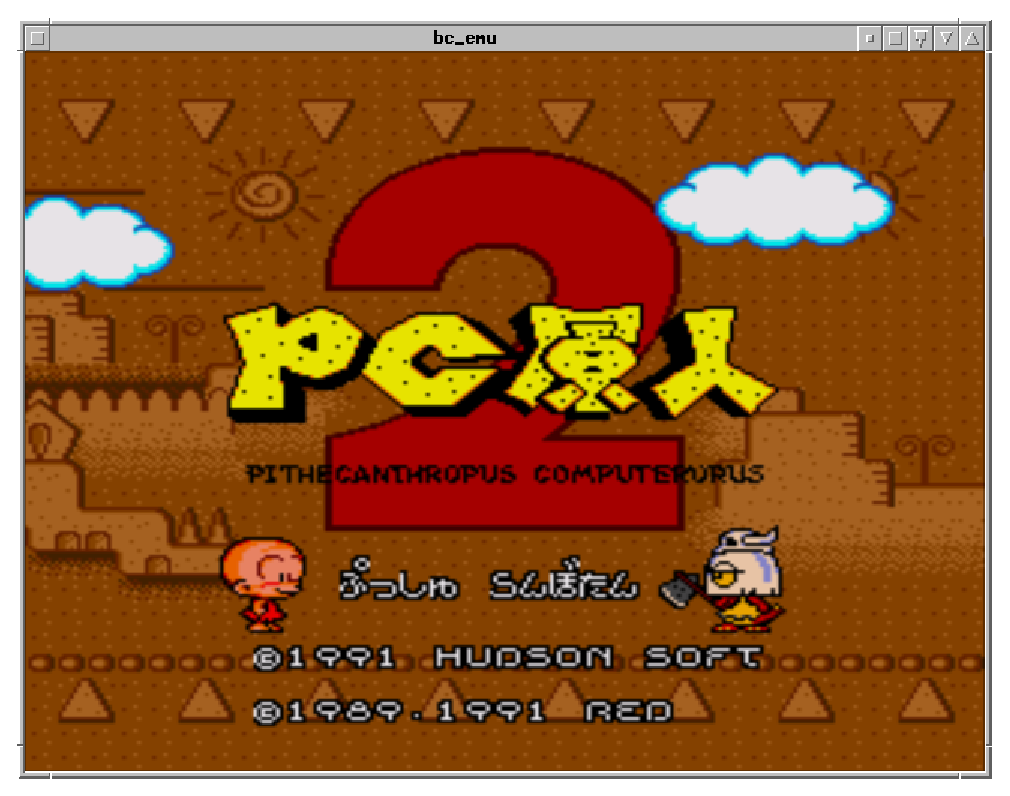
\includegraphics[width=3.6cm]{fig/bc_emu_ss1}
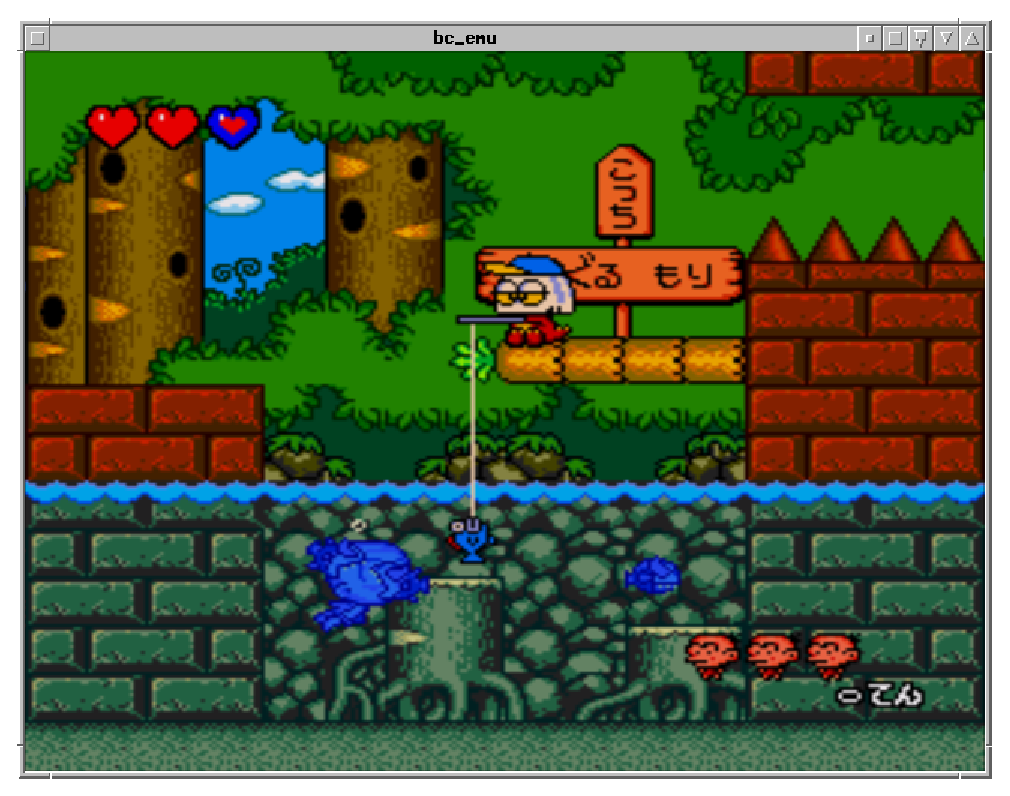
\includegraphics[width=3.6cm]{fig/bc_emu_ss2}
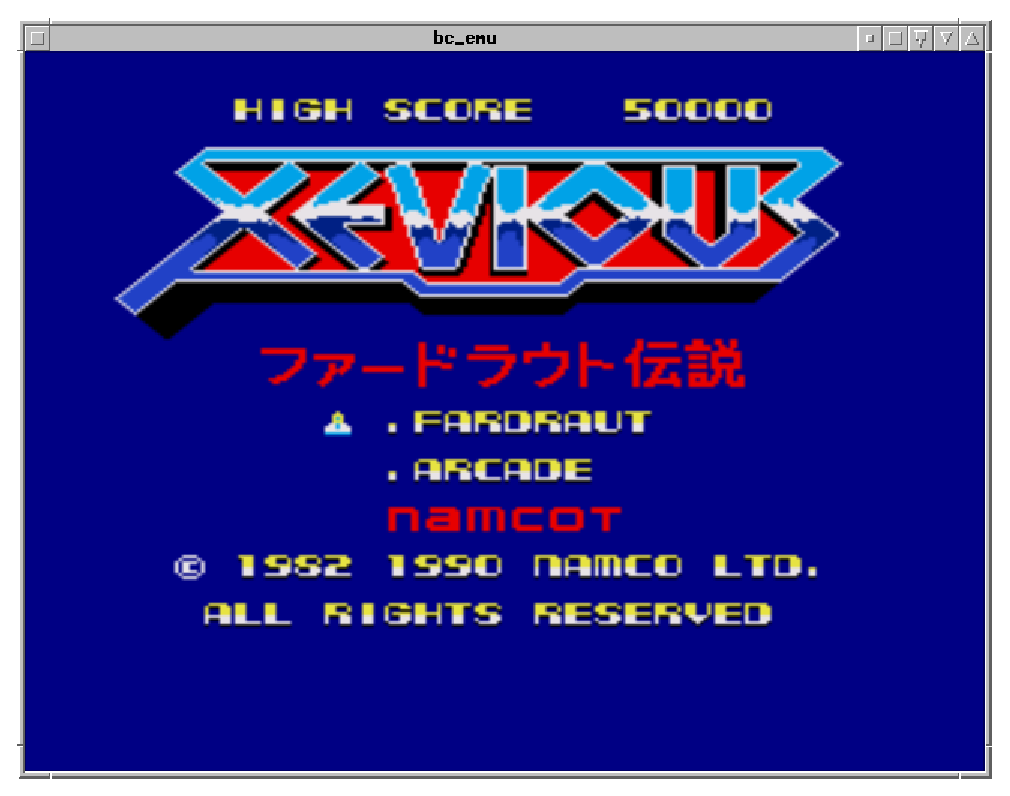
\includegraphics[width=3.6cm]{fig/bc_emu_ss3}
\end{frame}

% -----------------------------------------------------------------------------
% Conclusion/Summary
% -----------------------------------------------------------------------------
\section{Výsledky}

% Emulátor
\subsection{Naimplementovaný emulátor}
\begin{frame}
\frametitle{Naimplementovaný emulátor}
\begin{block}{Vlastnosti}
\begin{itemize}
	\item modul emulace systému NEC PCEngine
	\item moduly uživatelského rozhraní
	\begin{itemize}
		\item libSDL
		\item libSDL s grafikou akcelerovanou pomocí OpenGL
	\end{itemize}
	\item podporuje platformy
	\begin{itemize}
		\item {\em x86/x86\_64} - {\footnotesize GNU/Linux, Microsoft Windows}
		\item {\em ARM7/ARM9} - {\footnotesize Nintendo DS*}
	\end{itemize}
\end{itemize}
\end{block}
\vglue 2.5mm
\begin{center}
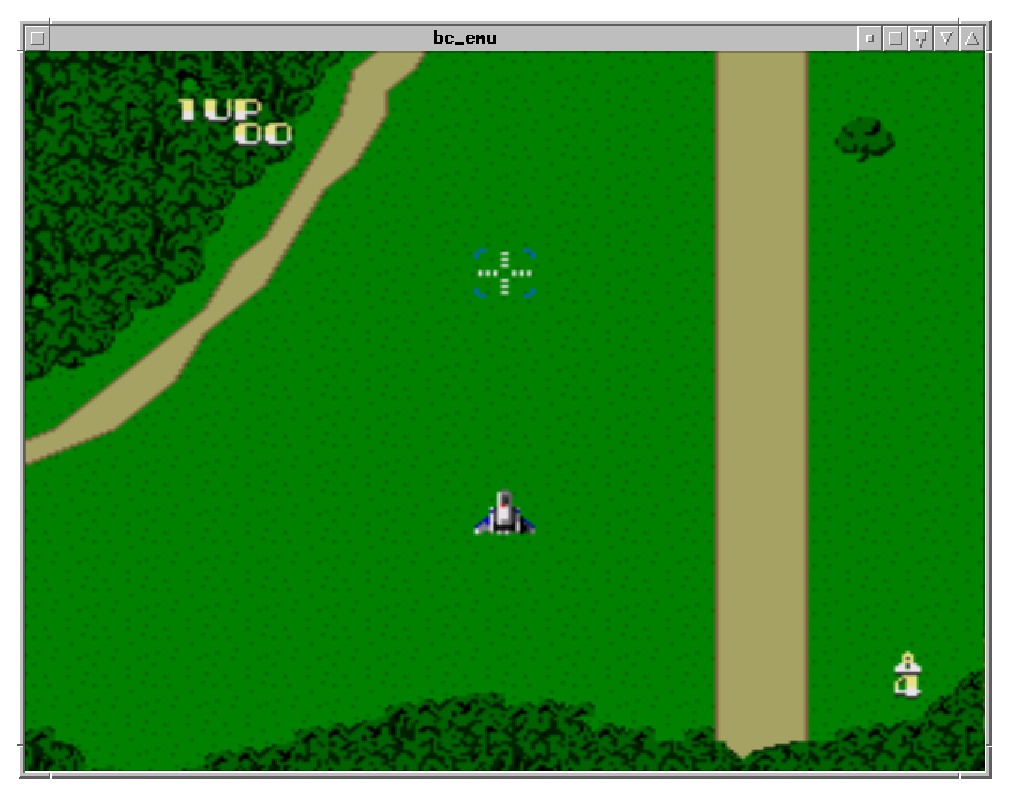
\includegraphics[width=3.6cm]{fig/bc_emu_ss4}
\end{center}
\end{frame}


% Vysledky
\subsection{Shrnutí výsledků práce}
\begin{frame}
\frametitle{Shrnutí výsledků práce}
% Vysledky prace
\begin{block}{Výsledky práce}
\begin{itemize}
	\item funkční emulátor systému NEC PCEngine
	\item testem ověřená podpora původních programů
	\item přenositelnost na úrovni zdrojového kódu podpořená:
	\begin{itemize}
		\item zvolenou architekturou programu
		\item použitím jazyka C
	\end{itemize}
	\item řada znovupoužitelných rutin pro interpretační emulaci
	\item rozšiřitelnost v oblasti uživ. rozhraní a emulovaných systémů
	\item ucelená dokumentace architektury NEC PCEngine
\end{itemize}
\end{block}
% Smer dalsiho vyvoje
\begin{block}{Směr dalšího vývoje}
\begin{itemize}
	\item nástroj pro lazení emulovaného programu
	\item zdokonalení kódu emulace PSG
	\item obecné konfigurační rozhraní
\end{itemize}
\end{block}

\end{frame}


\end{document}
